\documentclass[10pt]{article}
\usepackage[polish]{babel}
\usepackage[utf8]{inputenc}
\usepackage[T1]{fontenc}
\usepackage{graphicx}
\usepackage[export]{adjustbox}
\graphicspath{ {./images/} }
\usepackage{amsmath}
\usepackage{amsfonts}
\usepackage{amssymb}
\usepackage[version=4]{mhchem}
\usepackage{stmaryrd}

\title{Klasa }

\author{}
\date{}


\newcommand\Varangle{\mathop{{<\!\!\!\!\!\text{\small)}}\:}\nolimits}

\begin{document}
\maketitle
\begin{center}

\includegraphics[max width=\textwidth]{2024_11_21_597e779fde37da7a0aa4g-01}
\end{center}

Nazwisko i imię\\
MARZEC

PRÓBNY EGZAMIN MATURALNY Z MATEMATYKI

\section*{POZIOM PODSTAWOWY}
Czas pracy 170 minut

\section*{Instrukcja dla zdającego}
\begin{enumerate}
  \item Sprawdź, czy arkusz egzaminacyjny zawiera 22 strony (zadania 1-34).\\
Ewentualny brak zgłoś przewodniczącemu zespołu nadzorującego egzamin.
  \item Rozwiązania zadań i odpowiedzi wpisuj w miejscu na to przeznaczonym.
  \item Odpowiedzi do zadań zamkniętych (1-25) przenieś na kartę odpowiedzi, zaznaczając je w części karty przeznaczonej dla zdającego. Zamaluj pola do tego przeznaczone. Błędne zaznaczenie otocz kółkiem ( i zaznacz właściwe.
  \item Pamiętaj, że pominięcie argumentacji lub istotnych obliczeń w rozwiązaniu zadania otwartego (26-34) może spowodować, że za to rozwiązanie nie otrzymasz pełnej liczby punktów.
  \item Pisz czytelnie i używaj tylko długopisu lub pióra z czarnym tuszem lub atramentem.
  \item Nie używaj korektora, a błędne zapisy wyraźnie przekreśl.
  \item Pamiętaj, że zapisy w brudnopisie nie będą oceniane.
  \item Możesz korzystać z zestawu wzorów matematycznych, cyrkla, linijki oraz kalkulatora prostego.
  \item Nie wpisuj żadnych znaków w części przeznaczonej dla egzaminatora.
\end{enumerate}

Życzymy powodzenia!

Za rozwiązanie wszystkich zadań można otrzymać maksymalnie\\
50 punktów

\begin{center}
\begin{tabular}{c|c}
Życzymy powodzenia! &  \\
\hline
Prawa autorskie posiada Samorządowy Ośrodek Doradztwa Metodycznego i Doskonalenia &  \\
Nauczycieli w Kielcach &  \\
Kopiowanie w całości lub we fragmentach bez zgody wydawcy zabronione &  \\
\end{tabular}
\end{center}

\section*{ZADANIA ZAMKNIĘTE \\
 W zadaniach od 1. do 25. wybierz i zaznacz na karcie odpowiedzi poprawna odpowiedź.}
\section*{Zadanie 1. (0-1)}
Liczba \(\log _{2} 3-2 \log _{2} 4 \sqrt{3}\) jest równa\\
A. 4\\
B. -4\\
C. \(\frac{1}{4}\)\\
D. \(-\frac{1}{4}\)

\section*{Zadanie 2. (0-1)}
Liczba \(\sqrt[3]{2} \cdot \sqrt[3]{\frac{4}{27}}-1\) jest równa\\
A. \(\frac{2}{3}\)\\
B. \(-\frac{2}{3}\)\\
C. \(-\frac{1}{3}\)\\
D. \(\frac{1}{3}\)

\section*{Zadanie 3. (0-1)}
Dane są liczby \(a=1-3 \sqrt{2}\) oraz \(b=2+\sqrt{2}\). Wtedy iloraz liczb \(\frac{a}{b}\) jest równy\\
A. \(-2-7 \sqrt{2}\)\\
B. \(4-7 \sqrt{2}\)\\
C. \(-2-\frac{7}{2} \sqrt{2}\)\\
D. \(4-\frac{7}{2} \sqrt{2}\)

\section*{Zadanie 4. (0-1)}
Jeżeli w trójkącie prostokątnym jedną z przyprostokątnych zwiększymy o 10\%, a drugą zmniejszymy o \(10 \%\), to w wyniku obu przekształceń pole tego trójkąta\\
A. zwiększy się o \(1 \%\)\\
B. zmniejszy się o \(1 \%\)\\
C. nie zmieni się\\
D. zwiększy się o \(2 \%\)

\section*{Zadanie 5. (0-1)}
Liczba \(\frac{2^{20}}{4^{12}-8^{7}}\) jest równa\\
A. \(\frac{1}{14}\)\\
B. \(2^{17}\)\\
C. \(2^{15}\)\\
D. \(\frac{1}{32}\)

\section*{Zadanie 6. (0-1)}
Największą liczbą całkowitą należącą do zbioru rozwiązań nierówności \(\quad-2-\frac{3 x-4}{3} \geq x\) jest\\
A. -2\\
B. 0\\
C. 1\\
D. -1

\section*{BRUDNOPIS}
\begin{center}
\begin{tabular}{|c|c|c|c|c|c|c|c|c|c|c|c|c|c|c|c|c|c|c|c|c|c|c|}
\hline
 &  &  &  &  &  &  & - & - &  &  &  &  &  &  & - &  &  &  &  &  &  &  \\
\hline
 &  &  &  &  &  &  &  &  &  &  &  &  &  &  &  &  &  &  &  &  &  &  \\
\hline
 &  &  &  &  &  &  &  &  &  &  &  &  &  &  &  &  &  &  &  &  &  &  \\
\hline
 &  &  &  &  &  &  &  &  &  &  &  &  &  &  &  &  &  &  &  &  &  &  \\
\hline
 &  &  &  &  &  &  &  &  &  &  &  &  &  &  &  &  &  &  &  &  &  &  \\
\hline
 &  &  &  &  &  &  &  &  &  &  &  &  &  &  &  &  &  &  &  &  &  &  \\
\hline
 &  &  &  &  &  &  &  &  &  &  &  &  &  &  &  &  &  &  &  &  &  &  \\
\hline
 &  &  &  &  &  &  &  &  &  &  &  &  &  &  &  &  &  &  &  &  &  &  \\
\hline
 &  &  &  &  &  &  &  &  &  &  &  &  &  &  &  &  &  &  &  &  &  &  \\
\hline
 &  &  &  &  &  &  &  &  &  &  &  &  &  &  &  &  &  &  &  &  &  &  \\
\hline
 &  &  &  &  &  &  &  &  &  &  &  &  &  &  &  &  &  &  &  &  &  &  \\
\hline
 &  &  &  &  &  &  &  &  &  &  &  &  &  &  &  &  &  &  &  &  &  &  \\
\hline
 &  &  &  &  &  &  &  &  &  &  &  &  &  &  &  &  &  &  &  &  &  &  \\
\hline
 &  &  &  &  &  &  &  &  &  &  &  &  &  &  &  &  &  &  &  &  &  &  \\
\hline
 &  &  &  &  &  &  &  &  &  &  &  &  &  &  &  &  &  &  &  &  &  &  \\
\hline
 &  &  &  &  &  &  &  &  &  &  &  &  &  &  &  &  &  &  &  &  &  &  \\
\hline
 &  &  &  &  &  &  &  &  &  &  &  &  &  &  &  &  &  &  &  &  &  &  \\
\hline
 &  &  &  &  &  &  &  &  &  &  &  &  &  &  &  &  &  &  &  &  &  &  \\
\hline
 &  &  &  &  &  &  &  &  &  &  &  &  &  &  &  &  &  &  &  &  &  &  \\
\hline
 &  &  &  &  &  &  &  &  &  &  &  &  &  &  &  &  &  &  &  &  &  &  \\
\hline
 &  &  &  &  &  &  &  &  &  &  &  &  &  &  &  &  &  &  &  &  &  &  \\
\hline
 &  &  &  &  &  &  &  &  &  &  &  &  &  &  &  &  &  &  &  &  &  &  \\
\hline
 &  &  &  &  &  &  &  &  &  &  &  &  &  &  &  &  &  &  &  &  &  &  \\
\hline
 &  &  &  &  &  &  &  &  &  &  &  &  &  &  &  &  &  &  &  &  &  &  \\
\hline
 &  &  &  &  &  &  &  &  &  &  &  &  &  &  &  &  &  &  &  &  &  &  \\
\hline
 &  &  &  &  &  &  &  &  &  &  &  &  &  &  &  &  &  &  &  &  &  &  \\
\hline
 &  &  &  &  &  &  &  &  &  &  &  &  &  &  &  &  &  &  &  &  &  &  \\
\hline
 &  &  &  &  &  &  &  &  &  &  &  &  &  &  &  &  &  &  &  &  &  &  \\
\hline
 &  &  &  &  &  &  &  &  &  &  &  &  &  &  &  &  &  &  &  &  &  &  \\
\hline
 &  &  &  &  &  &  &  &  &  &  &  &  &  &  &  &  &  &  &  &  &  &  \\
\hline
 &  &  &  &  &  &  &  &  &  &  &  &  &  &  &  &  &  &  &  &  &  &  \\
\hline
 &  &  &  &  &  &  &  &  &  &  &  &  &  &  &  &  &  &  &  &  &  &  \\
\hline
 &  &  &  &  &  &  &  &  &  &  &  &  &  &  &  &  &  &  &  &  &  &  \\
\hline
 &  &  &  &  &  &  &  &  &  &  &  &  &  &  &  &  &  &  &  &  &  &  \\
\hline
 &  &  &  &  &  &  &  &  &  &  &  &  &  &  &  &  &  &  &  &  &  &  \\
\hline
 &  &  &  &  &  &  &  &  &  &  &  &  &  &  &  &  &  &  &  &  &  &  \\
\hline
 &  &  &  &  &  &  &  &  &  &  &  &  &  &  &  &  &  &  &  &  &  &  \\
\hline
 &  &  &  &  &  &  &  &  &  &  &  &  &  &  &  &  &  &  &  &  &  &  \\
\hline
 &  &  &  &  &  &  &  &  &  &  &  &  &  &  &  &  &  &  &  &  &  &  \\
\hline
 &  &  &  &  &  &  &  &  &  &  &  &  &  &  &  &  &  &  &  &  &  &  \\
\hline
 &  &  &  &  &  &  &  &  &  &  &  &  &  &  &  &  &  &  &  &  &  &  \\
\hline
 &  &  &  &  &  &  &  &  &  &  &  &  &  &  &  &  &  &  &  &  &  &  \\
\hline
 &  &  &  &  &  &  &  &  &  &  &  &  &  &  &  &  &  &  &  &  &  &  \\
\hline
 & - &  &  &  &  &  &  &  &  &  &  &  &  &  &  &  &  &  &  &  &  &  \\
\hline
\end{tabular}
\end{center}

\section*{Zadanie 7. (0-1)}
Miejscem zerowym funkcji \(f(x)=\frac{x+m}{2 m x-3}\) jest liczba -3 . Wtedy wartość \(m\) jest równa\\
A. 0\\
B. -3\\
C. 3\\
D. -2

\section*{Zadanie 8. (0-1)}
Funkcja \(f\) jest określona wzorem \(f(x)=(x-4)^{-\frac{1}{3}}\) dla każdej liczby rzeczywistej \(x \neq 4\). Wartość funkcji \(f\) dla argumentu -4 jest równa\\
A. \(\frac{1}{2}\)\\
B. 0\\
C. -2\\
D. \(-\frac{1}{2}\)

\section*{Zadanie 9. (0-1)}
Funkcja liniowa \(f(x)=\left(m^{2}-1\right) x+3 m-3\) ma nieskończenie wiele miejsc zerowych dla\\
A. \(m=1\)\\
B. \(m=-2\)\\
C. \(m=-1\)\\
D. \(m=0\)

\section*{Zadanie 10. (0-1)}
Punkt \(P=(-\sqrt{3}, 2)\) należy do wykresu funkcji \(f(x)=a x^{2}+2 \sqrt{3} x-4\). Wtedy współczynnik \(a\) jest równy\\
A. 0\\
B. \(\frac{\sqrt{3}}{10}\)\\
C. -4\\
D. 4

\section*{Zadanie 11. (0-1)}
Dana jest funkcja kwadratowa \(f(x)=-x^{2}+3 x+4\). Osią symetrii paraboli, która jest wykresem funkcji \(g(x)=f(-x)\) jest prosta o równaniu\\
A. \(x=-3\)\\
B. \(x=-\frac{3}{2}\)\\
C. \(y=\frac{25}{4}\)\\
D. \(x=\frac{3}{2}\)

\section*{Zadanie 12. (0-1)}
Liczby 2, 7, \(2 x-4\) w podanej kolejności są trzema kolejnymi wyrazami ciągu arytmetycznego, zatem \(x\) jest równy\\
A. 12\\
B. 8\\
C. 10\\
D. 16

\section*{Zadanie 13. (0-1)}
W ciągu geometrycznym \(\left(a_{n}\right)\) pierwszy wyraz \(a_{1}=3\) oraz \(a_{1}+a_{4}=84\). Iloraz tego ciągu jest równy\\
A. 3\\
B. 9\\
C. -3\\
D. 4

\section*{BRUDNOPIS}
\(\frac{4}{4}\)

\section*{Zadanie 14. (0-1)}
Kąt \(\alpha\) jest ostry oraz \(\operatorname{tg} \alpha=3\). Wartość wyrażenia \(\frac{2 \sin \alpha-3 \cos \alpha}{4 \cos \alpha}\) jest równa\\
A. 1\\
B. \(-\frac{1}{4}\)\\
C. \(\frac{9}{4}\)\\
D. \(\frac{3}{4}\)

\section*{Zadanie 15. (0-1)}
Na rysunku przedstawiony jest trójkąt prostokątny. Miara kąta \(\alpha\) spełnia warunek\\
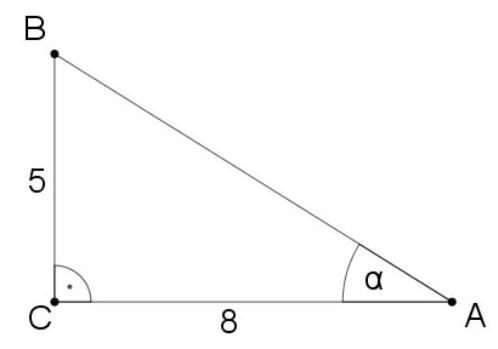
\includegraphics[max width=\textwidth, center]{2024_11_21_597e779fde37da7a0aa4g-06(1)}\\
A. \(\alpha \in\left(28^{\circ} ; 29^{\circ}\right)\)\\
B. \(\alpha>38^{\circ}\)\\
C. \(\alpha<28^{\circ}\)\\
D. \(\alpha \in\left(32^{\circ} ; 33^{\circ}\right)\)

\section*{Zadanie 16. (0-1)}
Na rysunku przedstawiona jest styczna \(k\) do okręgu o środku \(S\). Miara kąta \(\alpha\) jest równa\\
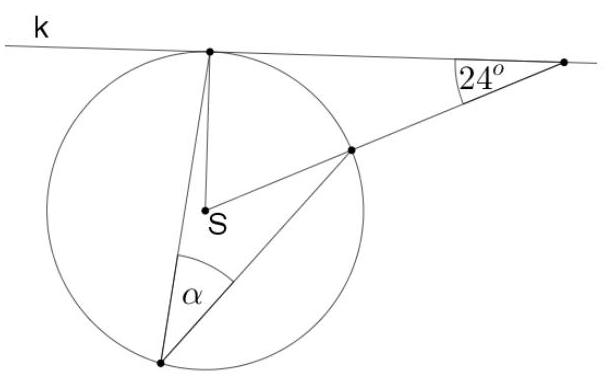
\includegraphics[max width=\textwidth, center]{2024_11_21_597e779fde37da7a0aa4g-06}\\
A. \(33^{\circ}\)\\
B. \(24^{\circ}\)\\
C. \(34^{\circ}\)\\
D. \(66^{\circ}\)

\section*{Zadanie 17. (0-1)}
Punkt \(\quad P\) leży na prostej o równaniu \(\quad y=-1 \frac{1}{2} x+4\). Zatem współrzędne punktu \(P\) mogą być równe\\
A. \((-16,27)\)\\
B. \((-30,50)\)\\
C. \((18,-21)\)\\
D. \((-40,64)\)

\section*{Zadanie 18. (0-1)}
Przekątne \(A C\) oraz \(B D\) równoległoboku \(A B C D\) przecinają się w punkcie \(S=\left(1,-\frac{1}{2}\right)\) Punkt \(A=(-3,-4)\), zatem\\
A. \(C=\left(5,4 \frac{1}{2}\right)\)\\
B. \(C=(6,3)\)\\
C. \(C=\left(-7,-7 \frac{1}{2}\right)\)\\
D. \(C=(5,3)\)

\section*{BRUDNOPIS}
\(\frac{4}{4}\)

\section*{Zadanie 19. (0-1)}
Proste o równaniach \(y=(2 m-3) x+4 m-1\) oraz \(y=-2 x+3 m-1\) są prostopadłe, gdy\\
A. \(m=1 \frac{3}{4}\)\\
B. \(m=-2 \frac{1}{2}\)\\
C. \(m=2 \frac{1}{2}\)\\
D. \(m=\frac{1}{2}\)

\section*{Zadanie 20. (0-1)}
Podstawą ostrosłupa jest trójkąt równoboczny \(A B C\). Punkty \(D\) i \(E\) są środkami odcinków \(A B\) oraz \(B C\). Wysokością tego ostrosłupa jest odcinek \(S D\), którego długość jest równa długości krawędzi podstawy (zobacz rysunek).\\
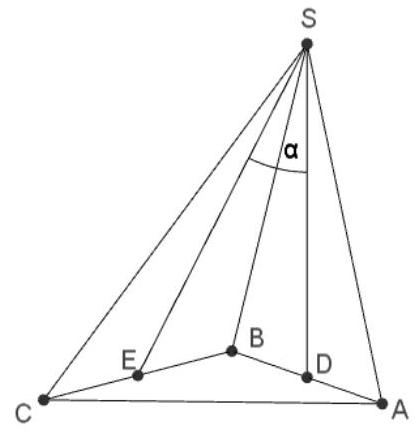
\includegraphics[max width=\textwidth, center]{2024_11_21_597e779fde37da7a0aa4g-08}

Kąt \(\alpha\), jaki tworzą odcinki \(S D\) oraz \(S E\), spełnia warunek\\
A. \(\alpha=30^{\circ}\)\\
B. \(\sin \alpha=\frac{1}{2}\)\\
C. \(\operatorname{tg} \alpha=\frac{1}{2}\)\\
D. \(\frac{1}{3}<\operatorname{tg} \alpha<\frac{1}{2}\)

\section*{Zadanie 21. (0-1)}
Prostopadłościan ma wymiary przedstawione na rysunku \(\left(|A B|=6,|B C|=4,\left|B B^{\prime}\right|=5\right)\).\\
Punkty \(E\) i \(F\) są środkami krawędzi \(A A^{\prime}\) oraz \(D D^{\prime}\).\\
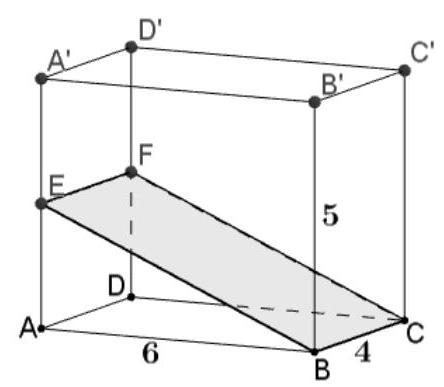
\includegraphics[max width=\textwidth, center]{2024_11_21_597e779fde37da7a0aa4g-08(1)}

Pole czworokąta \(B C F E\) jest równe\\
A. \(2 \sqrt{119}\)\\
B. 26\\
C. 28\\
D. 32

\section*{BRUDNOPIS}
\(\frac{4}{4}\)

\section*{Zadanie 22. (0-1)}
Na rysunku przedstawiono bryłę zbudowaną z walca i dwóch stożków. Przekroje osiowe stożków są trójkątami równobocznymi o boku 4, a wysokość walca jest równa 2.\\
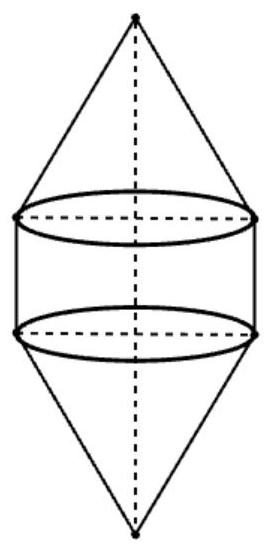
\includegraphics[max width=\textwidth, center]{2024_11_21_597e779fde37da7a0aa4g-10}

Pole powierzchni tej bryły jest równe\\
A. \(40 \pi\)\\
B. \(32 \pi\)\\
C. \(24 \pi\)\\
D. \(16 \pi(\sqrt{3}+1)\)

\section*{Zadanie 23. (0-1)}
Marek otrzymał następujące oceny z matematyki: \(3,3,4,6, x\). Średnia arytmetyczna tych ocen jest równa 4. Zatem ocena \(x\) to\\
A. 2\\
B. 3\\
C. 4\\
D. 5

\section*{Zadanie 24. (0-1)}
W pudełku jest 30 losów, w tym 5 wygrywających. Ile losów pustych należy usunaç z pudełka, aby losując jeden los prawdopodobieństwo wygranej było równe \(\frac{1}{5}\).\\
A. 6\\
B. 5\\
C. 8\\
D. 10

\section*{Zadanie 25. (0-1)}
Ze zbioru \(\{1,2,7,9,13,17,34\}\) losujemy jedną liczbę. Jakie jest prawdopodobieństwo wylosowania liczby pierwszej.\\
A. \(\frac{4}{7}\)\\
B. \(\frac{5}{7}\)\\
C. \(\frac{3}{7}\)\\
D. \(\frac{2}{7}\)

\section*{BRUDNOPIS}
\begin{center}

\includegraphics[max width=\textwidth]{2024_11_21_597e779fde37da7a0aa4g-11}
\end{center}

\section*{ZADANIA OTWARTE}
Rozwiazania zadań o numerach od 26. do 34. należy zapisać \(\boldsymbol{w}\) wyznaczonych miejscach pod treścia zadania.

\section*{Zadanie 26. (0-2)}
Rozwiąż nierówność \(x^{2}+2 x \leq 3(2 x-1)\).

\begin{center}
\begin{tabular}{|c|c|c|c|c|c|c|c|c|c|c|c|c|c|c|c|c|c|c|c|c|c|}
\hline
 &  & - & - & - & - & \textbackslash  & -" & \textbackslash  & - & \textbackslash  & - & \textbackslash  & \textbackslash  & | & ( &  & - \({ }^{-1}\) & [|. &  &  &  \\
\hline
 &  &  &  &  &  &  &  &  &  &  &  &  &  &  &  &  &  &  &  &  &  \\
\hline
 &  &  &  &  &  &  &  &  &  &  &  &  &  &  &  &  &  &  &  &  &  \\
\hline
 &  &  &  &  &  &  &  &  &  &  &  &  &  &  &  &  &  &  &  &  &  \\
\hline
 &  &  &  &  &  &  &  &  &  &  &  &  &  &  &  &  &  &  &  &  &  \\
\hline
 &  &  &  &  &  &  &  &  &  &  &  &  &  &  &  &  &  &  &  &  &  \\
\hline
 &  &  &  &  &  &  &  &  &  &  &  &  &  &  &  &  &  &  &  &  &  \\
\hline
 &  &  &  &  &  &  &  &  &  &  &  &  &  &  &  &  &  &  &  &  &  \\
\hline
 &  &  &  &  &  &  &  &  &  &  &  &  &  &  &  &  &  &  &  &  &  \\
\hline
 &  &  &  &  &  &  &  &  &  &  &  &  &  &  &  &  &  &  &  &  &  \\
\hline
 &  &  &  &  &  &  &  &  &  &  &  &  &  &  &  &  &  &  &  &  &  \\
\hline
 &  &  &  &  &  &  &  &  &  &  &  &  &  &  &  &  &  &  &  &  &  \\
\hline
 &  &  &  &  &  &  &  &  &  &  &  &  &  &  &  &  &  &  &  &  &  \\
\hline
 &  &  &  &  &  &  &  &  &  &  &  &  &  &  &  &  &  &  &  &  &  \\
\hline
 &  &  &  &  &  &  &  &  &  &  &  &  &  &  &  &  &  &  &  &  &  \\
\hline
 &  &  &  &  &  &  &  &  &  &  &  &  &  &  &  &  &  &  &  &  &  \\
\hline
 &  &  &  &  &  &  &  &  &  &  &  &  &  &  &  &  &  &  &  &  &  \\
\hline
 &  &  &  &  &  &  &  &  &  &  &  &  &  &  &  &  &  &  &  &  &  \\
\hline
 &  &  &  &  &  &  &  &  &  &  &  &  &  &  &  &  &  &  &  &  &  \\
\hline
 &  &  &  &  &  &  &  &  &  &  &  &  &  &  &  &  &  &  &  &  &  \\
\hline
 &  &  &  &  &  &  &  &  &  &  &  &  &  &  &  &  &  &  &  &  &  \\
\hline
 &  &  &  &  &  &  &  &  &  &  &  &  &  &  &  &  &  &  &  &  &  \\
\hline
 &  &  &  &  &  &  &  &  &  &  &  &  &  &  &  &  &  &  &  &  &  \\
\hline
 &  &  &  &  &  &  &  &  &  &  &  &  &  &  &  &  &  &  &  &  &  \\
\hline
 &  &  &  &  &  &  &  &  &  &  &  &  &  &  &  &  &  &  &  &  &  \\
\hline
 &  &  &  &  &  &  &  &  &  &  &  &  &  &  &  &  &  &  &  &  &  \\
\hline
 &  &  &  &  &  &  &  &  &  &  &  &  &  &  &  &  &  &  &  &  &  \\
\hline
 &  &  &  &  &  &  &  &  &  &  &  &  &  &  &  &  &  &  &  &  &  \\
\hline
 &  &  &  &  &  &  &  &  &  &  &  &  &  &  &  &  &  &  &  &  &  \\
\hline
 &  &  &  &  &  &  &  &  &  &  &  &  &  &  &  &  &  &  &  &  &  \\
\hline
 &  &  &  &  &  &  &  &  &  &  &  &  &  &  &  &  &  &  &  &  &  \\
\hline
 &  &  &  &  &  &  &  &  &  &  &  &  &  &  &  &  &  &  &  &  &  \\
\hline
 &  &  &  &  &  &  &  &  &  &  &  &  &  &  &  &  &  &  &  &  &  \\
\hline
 &  &  &  &  &  &  &  &  &  &  &  &  &  &  &  &  &  &  &  &  &  \\
\hline
 &  &  &  &  &  &  &  &  &  &  &  &  &  &  &  &  &  &  &  &  &  \\
\hline
 &  &  &  &  &  &  &  &  &  &  &  &  &  &  &  &  &  &  &  &  &  \\
\hline
 &  &  &  &  &  &  &  &  &  &  &  &  &  &  &  &  &  &  &  &  &  \\
\hline
\end{tabular}
\end{center}

Zadanie 27. (0-2)\\
Rozwiąż równanie \((2 x-1)\left(x^{3}+8\right)\left(x^{2}+9\right)=0\).\\

\includegraphics[max width=\textwidth, center]{2024_11_21_597e779fde37da7a0aa4g-13}

\section*{Zadanie 28. (0-2)}
Udowodnij, że dla dowolnych liczb rzeczywistych dodatnich \(x\) i \(y\) prawdziwa jest nierówność

\[
\frac{x}{y} \geq 4\left(1-\frac{y}{x}\right)
\]

\begin{center}
\begin{tabular}{|c|c|c|c|c|c|c|c|c|c|c|c|c|c|c|c|c|c|c|c|c|c|c|c|c|c|c|c|c|c|c|}
\hline
 &  &  &  &  &  &  &  &  &  &  &  &  &  &  &  &  &  &  &  &  &  &  &  &  &  &  &  &  &  &  \\
\hline
 &  &  &  &  &  &  &  &  &  &  &  &  &  &  &  &  &  &  &  &  &  &  &  &  &  &  &  &  &  &  \\
\hline
 &  &  &  &  &  &  &  &  &  &  &  &  &  &  &  &  &  &  &  &  &  &  &  &  &  &  &  &  &  &  \\
\hline
 &  &  &  &  &  &  &  &  &  &  &  &  &  &  &  &  &  &  &  &  &  &  &  &  &  &  &  &  &  &  \\
\hline
 &  &  &  &  &  &  &  &  &  &  &  &  &  &  &  &  &  &  &  &  &  &  &  &  &  &  &  &  &  &  \\
\hline
 &  &  &  &  &  &  &  &  &  &  &  &  &  &  &  &  &  &  &  &  &  &  &  &  &  &  &  &  &  &  \\
\hline
 &  &  &  &  &  &  &  &  &  &  &  &  &  &  &  &  &  &  &  &  &  &  &  &  &  &  &  &  &  &  \\
\hline
 &  &  &  &  &  &  &  &  &  &  &  &  &  &  &  &  &  &  &  &  &  &  &  &  &  &  &  &  &  &  \\
\hline
 &  &  &  &  &  &  &  &  &  &  &  &  &  &  &  &  &  &  &  &  &  &  &  &  &  &  &  &  &  &  \\
\hline
 &  &  &  &  &  &  &  &  &  &  &  &  &  &  &  &  &  &  &  &  &  &  &  &  &  &  &  &  &  &  \\
\hline
 &  &  &  &  &  &  &  &  &  &  &  &  &  &  &  &  &  &  &  &  &  &  &  &  &  &  &  &  &  &  \\
\hline
 &  &  &  &  &  &  &  &  &  &  &  &  &  &  &  &  &  &  &  &  &  &  &  &  &  &  &  &  &  &  \\
\hline
 &  &  &  &  &  &  &  &  &  &  &  &  &  &  &  &  &  &  &  &  &  &  &  &  &  &  &  &  &  &  \\
\hline
 &  &  &  &  &  &  &  &  &  &  &  &  &  &  &  &  &  &  &  &  &  &  &  &  &  &  &  &  &  &  \\
\hline
 &  &  &  &  &  &  &  &  &  &  &  &  &  &  &  &  &  &  &  &  &  &  &  &  &  &  &  &  &  &  \\
\hline
 &  &  &  &  &  &  &  &  &  &  &  &  &  &  &  &  &  &  &  &  &  &  &  &  &  &  &  &  &  &  \\
\hline
 &  &  &  &  &  &  &  &  &  &  &  &  &  &  &  &  &  &  &  &  &  &  &  &  &  &  &  &  &  &  \\
\hline
 &  &  &  &  &  &  &  &  &  &  &  &  &  &  &  &  &  &  &  &  &  &  &  &  &  &  &  &  &  &  \\
\hline
 &  &  &  &  &  &  &  &  &  &  &  &  &  &  &  &  &  &  &  &  &  &  &  &  &  &  &  &  &  &  \\
\hline
 &  &  &  &  &  &  &  &  &  &  &  &  &  &  &  &  &  &  &  &  &  &  &  &  &  &  &  &  &  &  \\
\hline
 &  &  &  &  &  &  &  &  &  &  &  &  &  &  &  &  &  &  &  &  &  &  &  &  &  &  &  &  &  &  \\
\hline
 &  &  &  &  &  &  &  &  &  &  &  &  &  &  &  &  &  &  &  &  &  &  &  &  &  &  &  &  &  &  \\
\hline
 &  &  &  &  &  &  &  &  &  &  &  &  &  &  &  &  &  &  &  &  &  &  &  &  &  &  &  &  &  &  \\
\hline
 &  &  &  &  &  &  &  &  &  &  &  &  &  &  &  &  &  &  &  &  &  &  &  &  &  &  &  &  &  &  \\
\hline
 &  &  &  &  &  &  &  &  &  &  &  &  &  &  &  &  &  &  &  &  &  &  &  &  &  &  &  &  &  &  \\
\hline
 &  &  &  &  &  &  &  &  &  &  &  &  &  &  &  &  &  &  &  &  &  &  &  &  &  &  &  &  &  &  \\
\hline
 &  &  &  &  &  &  &  &  &  &  &  &  &  &  &  &  &  &  &  &  &  &  &  &  &  &  &  &  &  &  \\
\hline
 &  &  &  &  &  &  &  &  &  &  &  &  &  &  &  &  &  &  &  &  &  &  &  &  &  &  &  &  &  &  \\
\hline
 &  &  &  &  &  &  &  &  &  &  &  &  &  &  &  &  &  &  &  &  &  &  &  &  &  &  &  &  &  &  \\
\hline
 &  &  &  &  &  &  &  &  &  &  &  &  &  &  &  &  &  &  &  &  &  &  &  &  &  &  &  &  &  &  \\
\hline
 &  &  &  &  &  &  &  &  &  &  &  &  &  &  &  &  &  &  &  &  &  &  &  &  &  &  &  &  &  &  \\
\hline
 &  &  &  &  &  &  &  &  &  &  &  &  &  &  &  &  &  &  &  &  &  &  &  &  &  &  &  &  &  &  \\
\hline
 &  &  &  &  &  &  &  &  &  &  &  &  &  &  &  &  &  &  &  &  &  &  &  &  &  &  &  &  &  &  \\
\hline
 &  &  &  &  &  &  &  & - &  &  &  &  &  &  &  &  &  &  &  &  &  &  &  &  &  &  &  &  &  &  \\
\hline
 &  &  &  &  &  &  &  &  &  &  &  &  &  &  &  &  &  &  &  &  &  &  &  &  &  &  &  &  &  &  \\
\hline
 &  &  &  &  &  &  &  &  &  &  &  &  &  &  &  &  &  &  &  &  &  &  &  &  &  &  &  &  &  &  \\
\hline
 &  &  &  &  &  &  &  &  &  &  &  &  &  &  &  &  &  &  &  &  &  &  &  &  &  &  &  &  &  &  \\
\hline
 &  &  &  &  &  &  &  &  &  &  &  &  &  &  &  &  &  &  &  &  &  &  &  &  &  &  &  &  &  &  \\
\hline
\end{tabular}
\end{center}

Odpowiedź.

\section*{Zadanie 29. (0-2)}
W równoległoboku \(A B C D\) poprowadzono odcinek KM. Punkt M jest środkiem odcinka \(A B\), punkt K leży na odcinku CD oraz 2 \(|\mathrm{DK}|=|\mathrm{KC}|\) (zobacz rysunek). Uzasadnij, że stosunek pola trapezu AMKD do pola trapezu MBCK jest równy \(\frac{5}{7}\).\\
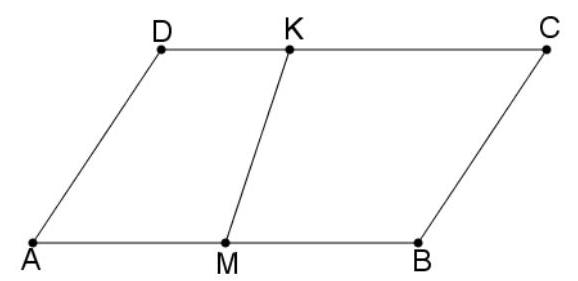
\includegraphics[max width=\textwidth, center]{2024_11_21_597e779fde37da7a0aa4g-15}

\begin{center}
\begin{tabular}{|c|c|c|c|c|c|c|c|c|c|c|c|c|c|c|c|c|c|c|c|c|c|c|c|c|c|c|c|c|c|c|}
\hline
 &  &  &  &  &  &  &  &  &  &  &  &  &  &  &  &  &  &  &  &  &  &  &  &  &  &  &  &  &  &  \\
\hline
 &  &  &  &  &  &  &  &  &  &  &  &  &  &  &  &  &  &  &  &  &  &  &  &  &  &  &  &  &  &  \\
\hline
 &  &  &  &  &  &  &  &  &  &  &  &  &  &  &  &  &  &  &  &  &  &  &  &  &  &  &  &  &  &  \\
\hline
 &  &  &  &  &  &  &  &  &  &  &  &  &  &  &  &  &  &  &  &  &  &  &  &  &  &  &  &  &  &  \\
\hline
 &  &  &  &  &  &  &  &  &  &  &  &  &  &  &  &  &  &  &  &  &  &  &  &  &  &  &  &  &  &  \\
\hline
 &  &  &  &  &  &  &  &  &  &  &  &  &  &  &  &  &  &  &  &  &  &  &  &  &  &  &  &  &  &  \\
\hline
 &  &  &  &  &  &  &  &  &  &  &  &  &  &  &  &  &  &  &  &  &  &  &  &  &  &  &  &  &  &  \\
\hline
 &  &  &  &  &  &  &  &  &  &  &  &  &  &  &  &  &  &  &  &  &  &  &  &  &  &  &  &  &  &  \\
\hline
 &  &  &  &  &  &  &  &  &  &  &  &  &  &  &  &  &  &  &  &  &  &  &  &  &  &  &  &  &  &  \\
\hline
 &  &  &  &  &  &  &  &  &  &  &  &  &  &  &  &  &  &  &  &  &  &  &  &  &  &  &  &  &  &  \\
\hline
 &  &  &  &  &  &  &  &  &  &  &  &  &  &  &  &  &  &  &  &  &  &  &  &  &  &  &  &  &  &  \\
\hline
 &  &  &  &  &  &  &  &  &  &  &  &  &  &  &  &  &  &  &  &  &  &  &  &  &  &  &  &  &  &  \\
\hline
 &  &  &  &  &  &  &  &  &  &  &  &  &  &  &  &  &  &  &  &  &  &  &  &  &  &  &  &  &  &  \\
\hline
 &  &  &  &  &  &  &  &  &  &  &  &  &  &  &  &  &  &  &  &  &  &  &  &  &  &  &  &  &  &  \\
\hline
 &  &  &  &  &  &  &  &  &  &  &  &  &  &  &  &  &  &  &  &  &  &  &  &  &  &  &  &  &  &  \\
\hline
 &  &  &  &  &  &  &  &  &  &  &  &  &  &  &  &  &  &  &  &  &  &  &  &  &  &  &  &  &  &  \\
\hline
 &  &  &  &  &  &  &  &  &  &  &  &  &  &  &  &  &  &  &  &  &  &  &  &  &  &  &  &  &  &  \\
\hline
 &  &  &  &  &  &  &  &  &  &  &  &  &  &  &  &  &  &  &  &  &  &  &  &  &  &  &  &  &  &  \\
\hline
 &  &  &  &  &  &  &  &  &  &  &  &  &  &  &  &  &  &  &  &  &  &  &  &  &  &  &  &  &  &  \\
\hline
 &  &  &  &  &  &  &  &  &  &  &  &  &  &  &  &  &  &  &  &  &  &  &  &  &  &  &  &  &  &  \\
\hline
 &  &  &  &  &  &  &  &  &  &  &  &  &  &  &  &  &  &  &  &  &  &  &  &  &  &  &  &  &  &  \\
\hline
 &  &  &  &  &  &  &  &  &  &  &  &  &  &  &  &  &  &  &  &  &  &  &  &  &  &  &  &  &  &  \\
\hline
 &  &  &  &  &  &  &  &  &  &  &  &  &  &  &  &  &  &  &  &  &  &  &  &  &  &  &  &  &  &  \\
\hline
 &  &  &  &  &  &  &  &  &  &  &  &  &  &  &  &  &  &  &  &  &  &  &  &  &  &  &  &  &  &  \\
\hline
 &  &  &  &  &  &  &  &  &  &  &  &  &  &  &  &  &  &  &  &  &  &  &  &  &  &  &  &  &  &  \\
\hline
 &  &  &  &  &  &  &  &  &  &  &  &  &  &  &  &  &  &  &  &  &  &  &  &  &  &  &  &  &  &  \\
\hline
 &  &  &  &  &  &  &  &  &  &  &  &  &  &  &  &  &  &  &  &  &  &  &  &  &  &  &  &  &  &  \\
\hline
 &  &  &  &  &  &  &  &  &  &  &  &  &  &  &  &  &  &  &  &  &  &  &  &  &  &  &  &  &  &  \\
\hline
 &  &  &  &  &  &  &  &  &  &  &  &  &  &  &  &  &  &  &  &  &  &  &  &  &  &  &  &  &  &  \\
\hline
 &  &  &  &  &  &  &  &  &  &  &  &  &  &  &  &  &  &  &  &  &  &  &  &  &  & ......... &  &  &  &  \\
\hline
 & , &  &  &  &  &  &  &  &  &  &  &  &  &  &  &  &  &  &  &  &  &  &  &  &  &  &  &  &  &  \\
\hline
 &  &  &  &  &  &  &  &  &  &  &  &  &  &  &  &  &  &  &  &  &  &  &  &  &  & \(\qquad\) &  &  &  &  \\
\hline
 & , &  &  &  &  &  &  &  &  &  &  &  &  &  &  &  &  &  &  &  &  &  &  &  &  &  &  &  &  &  \\
\hline
 &  &  &  &  &  &  &  &  &  &  &  &  &  &  &  &  &  &  &  &  &  &  &  &  &  &  &  &  &  &  \\
\hline
\end{tabular}
\end{center}

Zadanie 30. (0-2)\\
Ze zbioru liczb naturalnych trzycyfrowych losujemy jedną liczbę. Jakie jest prawdopodobieństwo, że suma cyfr wylosowanej liczby jest równa 5.\\

\includegraphics[max width=\textwidth, center]{2024_11_21_597e779fde37da7a0aa4g-16}

Odpowiedź.

\section*{Zadanie 31. (0-2)}
Suma trzech początkowych wyrazów \(a_{1}+a_{2}+a_{3}\) ciągu arytmetycznego \(\left(a_{n}\right)\) jest o 18 większa od sumy \(a_{4}+a_{5}+a_{6}\). Wyznacz różnicę \(r\) tego ciągu.\\

\includegraphics[max width=\textwidth, center]{2024_11_21_597e779fde37da7a0aa4g-17}

\section*{Zadanie 32. (0-4)}
Punkty \(A=\left(-1,3 \frac{1}{2}\right)\) oraz \(B=(4,6)\) należą do wykresu funkcji \(f(x)=-\frac{1}{2} x^{2}+b x+c\).\\
Wyznacz wartości liczbowe współczynników \(b\) i \(c\). Dla wyznaczonych wartości \(b\) oraz \(c\) oblicz pole trójkąta, którego wierzchołkami są punkty przecięcia wykresu funkcji \(f \mathrm{z}\) osiami układu współrzędnych.

\begin{center}
\begin{tabular}{|c|c|c|c|c|c|c|c|c|c|c|c|c|c|c|c|c|c|c|c|c|c|c|c|c|c|c|c|c|c|c|}
\hline
 &  &  &  &  &  &  &  &  &  &  &  &  &  &  &  &  &  &  &  &  &  &  &  &  &  &  &  &  &  &  \\
\hline
 &  &  &  &  &  &  &  &  &  &  &  &  &  &  &  &  &  &  &  &  &  &  &  &  &  &  &  &  &  &  \\
\hline
 &  &  &  &  &  &  &  &  &  &  &  &  &  &  &  &  &  &  &  &  &  &  &  &  &  &  &  &  &  &  \\
\hline
 &  &  &  &  &  &  &  &  &  &  &  &  &  &  &  &  &  &  &  &  &  &  &  &  &  &  &  &  &  &  \\
\hline
 &  &  &  &  &  &  &  &  &  &  &  &  &  &  &  &  &  &  &  &  &  &  &  &  &  &  &  &  &  &  \\
\hline
 &  &  &  &  &  &  &  &  &  &  &  &  &  &  &  &  &  &  &  &  &  &  &  &  &  &  &  &  &  &  \\
\hline
 &  &  &  &  &  &  &  &  &  &  &  &  &  &  &  &  &  &  &  &  &  &  &  &  &  &  &  &  &  &  \\
\hline
 &  &  &  &  &  &  &  &  &  &  &  &  &  &  &  &  &  &  &  &  &  &  &  &  &  &  &  &  &  &  \\
\hline
 &  &  &  &  &  &  &  &  &  &  &  &  &  &  &  &  &  &  &  &  &  &  &  &  &  &  &  &  &  &  \\
\hline
 &  &  &  &  &  &  &  &  &  &  &  &  &  &  &  &  &  &  &  &  &  &  &  &  &  &  &  &  &  &  \\
\hline
 &  &  &  &  &  &  &  &  &  &  &  &  &  &  &  &  &  &  &  &  &  &  &  &  &  &  &  &  &  &  \\
\hline
 &  &  &  &  &  &  &  &  &  &  &  &  &  &  &  &  &  &  &  &  &  &  &  &  &  &  &  &  &  &  \\
\hline
 &  &  &  &  &  &  &  &  &  &  &  &  &  &  &  &  &  &  &  &  &  &  &  &  &  &  &  &  &  &  \\
\hline
 &  &  &  &  &  &  &  &  &  &  &  &  &  &  &  &  &  &  &  &  &  &  &  &  &  &  &  &  &  &  \\
\hline
 &  &  &  &  &  &  &  &  &  &  &  &  &  &  &  &  &  &  &  &  &  &  &  &  &  &  &  &  &  &  \\
\hline
 &  &  &  &  &  &  &  &  &  &  &  &  &  &  &  &  &  &  &  &  &  &  &  &  &  &  &  &  &  &  \\
\hline
 &  &  &  &  &  &  &  &  &  &  &  &  &  &  &  &  &  &  &  &  &  &  &  &  &  &  &  &  &  &  \\
\hline
 &  &  &  &  &  &  &  &  &  &  &  &  &  &  &  &  &  &  &  &  &  &  &  &  &  &  &  &  &  &  \\
\hline
 &  &  &  &  &  &  &  &  &  &  &  &  &  &  &  &  &  &  &  &  &  &  &  &  &  &  &  &  &  &  \\
\hline
 &  &  &  &  &  &  &  &  &  &  &  &  &  &  &  &  &  &  &  &  &  &  &  &  &  &  &  &  &  &  \\
\hline
 &  &  &  &  &  &  &  &  &  &  &  &  &  &  &  &  &  &  &  &  &  &  &  &  &  &  &  &  &  &  \\
\hline
 &  &  &  &  &  &  &  &  &  &  &  &  &  &  &  &  &  &  &  &  &  &  &  &  &  &  &  &  &  &  \\
\hline
 &  &  &  &  &  &  &  &  &  &  &  &  &  &  &  &  &  &  &  &  &  &  &  &  &  &  &  &  &  &  \\
\hline
 &  &  &  &  &  &  &  &  &  &  &  &  &  &  &  &  &  &  &  &  &  &  &  &  &  &  &  &  &  &  \\
\hline
 &  &  &  &  &  &  &  &  &  & , &  &  &  &  &  &  &  &  &  &  &  &  &  &  &  &  &  &  &  &  \\
\hline
 &  &  &  &  &  &  &  &  &  &  &  &  &  &  &  &  &  &  &  &  &  &  &  &  &  &  &  &  &  &  \\
\hline
 &  &  &  &  & , &  &  &  &  & , &  &  &  &  &  &  &  &  &  &  &  &  &  &  &  &  &  &  &  &  \\
\hline
 &  &  &  &  &  &  &  &  &  &  &  &  &  &  &  &  &  &  &  &  &  &  &  &  &  &  &  &  &  &  \\
\hline
 &  &  &  &  &  &  &  &  &  &  &  &  &  &  &  &  &  &  &  &  &  &  &  &  &  &  &  &  &  &  \\
\hline
 &  &  &  &  &  &  &  &  &  &  &  &  &  &  &  &  &  &  &  &  &  &  &  &  &  &  &  &  &  &  \\
\hline
 &  &  &  &  &  &  &  &  &  &  &  &  &  &  &  &  &  &  &  &  &  &  &  &  &  &  &  &  &  &  \\
\hline
 &  &  &  &  & \textbackslash  &  &  &  &  &  &  &  & , & , &  &  &  &  &  &  &  &  &  &  &  &  &  &  &  &  \\
\hline
 &  &  &  &  &  &  &  &  &  &  &  &  &  & , &  &  &  &  &  &  &  &  &  &  &  &  &  &  &  &  \\
\hline
 &  &  &  &  &  &  &  &  &  &  &  &  &  &  &  &  &  &  &  &  &  &  &  &  &  &  &  &  &  &  \\
\hline
 &  &  &  &  &  &  &  &  &  &  &  &  &  &  &  &  &  &  &  &  &  &  &  &  &  &  &  &  &  &  \\
\hline
 &  &  &  &  &  &  &  &  &  &  &  &  &  &  &  &  &  &  &  &  &  &  &  &  &  &  &  &  &  &  \\
\hline
 &  &  &  &  &  &  &  &  &  &  &  &  &  &  &  &  &  &  &  &  &  &  &  &  &  &  &  &  &  &  \\
\hline
\end{tabular}
\end{center}

Odpowiedź.

\section*{Zadanie 33. (0-4)}
W trójkącie \(A B C\) miara kąta przy wierzchołku \(B\) jest równa \(90^{\circ}\), a wierzchołek \(A=(5,2)\). Punkty \(B\) i \(C\) leżą na prostej o równaniu \(y=3 x+6\), przy czym punkt \(C\) należy również do osi odciętych układu współrzędnych. Wyznacz współrzędne wierzchołków \(B\) i \(C\) oraz pole tego trójkąta.\\

\includegraphics[max width=\textwidth, center]{2024_11_21_597e779fde37da7a0aa4g-19}

Odpowiedź.

\section*{Zadanie 34. (0-5)}
Podstawą graniastostupa prostego jest trapez prostokątny \(A B C D\), w którym \(|B C|=4,|D C|=6\), \(|\Varangle B A D|=|\Varangle A D C|=90^{\circ}\) oraz \(|\Varangle A B C|=60^{\circ}\) (rysunek poniżej). Krótsza przekątna graniastosłupa \(A C^{\prime}\) ma długość \(4 \sqrt{7}\). Wyznacz pole powierzchni całkowitej oraz objętość graniastosłupa.\\
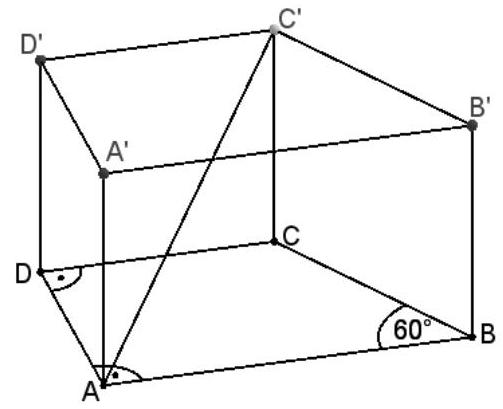
\includegraphics[max width=\textwidth, center]{2024_11_21_597e779fde37da7a0aa4g-20}

\begin{center}
\begin{tabular}{|c|c|c|c|c|c|c|c|c|c|c|c|c|c|c|c|c|c|c|c|c|c|c|c|c|c|c|c|c|c|c|}
\hline
 &  &  &  &  &  &  &  &  &  &  &  &  &  &  &  &  &  &  &  &  &  &  &  &  &  &  &  &  &  &  \\
\hline
 &  &  &  &  &  &  &  &  &  &  &  &  &  &  &  &  &  &  &  &  &  &  &  &  &  &  &  &  &  &  \\
\hline
 &  &  &  &  &  &  &  &  &  &  &  &  &  &  &  &  &  &  &  &  &  &  &  &  &  &  &  &  &  &  \\
\hline
 &  &  &  &  &  &  &  &  &  &  &  &  &  &  &  &  &  &  &  &  &  &  &  &  &  &  &  &  &  &  \\
\hline
 &  &  &  &  &  &  &  &  &  &  &  &  &  &  &  &  &  &  &  &  &  &  &  &  &  &  &  &  &  &  \\
\hline
 &  &  &  &  &  &  &  &  &  &  &  &  &  &  &  &  &  &  &  &  &  &  &  &  &  &  &  &  &  &  \\
\hline
 &  &  &  &  &  &  &  &  &  &  &  &  &  &  &  &  &  &  &  &  &  &  &  &  &  &  &  &  &  &  \\
\hline
 &  &  &  &  &  &  &  &  &  &  &  &  &  &  &  &  &  &  &  &  &  &  &  &  &  &  &  &  &  &  \\
\hline
 &  &  &  &  &  &  &  &  &  &  &  &  &  &  &  &  &  &  &  &  &  &  &  &  &  &  &  &  &  &  \\
\hline
 &  &  &  &  &  &  &  &  &  &  &  &  &  &  &  &  &  &  &  &  &  &  &  &  &  &  &  &  &  &  \\
\hline
 &  &  &  &  &  &  &  &  &  &  &  &  &  &  &  &  &  &  &  &  &  &  &  &  &  &  &  &  &  &  \\
\hline
 &  &  &  &  &  &  &  &  &  &  &  &  &  &  &  &  &  &  &  &  &  &  &  &  &  &  &  &  &  &  \\
\hline
 &  &  &  &  &  &  &  &  &  &  &  &  &  &  &  &  &  &  &  &  &  &  &  &  &  &  &  &  &  &  \\
\hline
 &  &  &  &  &  &  &  &  &  &  &  &  &  &  &  &  &  &  &  &  &  &  &  &  &  &  &  &  &  &  \\
\hline
 &  &  &  &  &  &  &  &  &  &  &  &  &  &  &  &  &  &  &  &  &  &  &  &  &  &  &  &  &  &  \\
\hline
 &  &  &  &  &  &  &  &  &  &  &  &  &  &  &  &  &  &  &  &  &  &  &  &  &  &  &  &  &  &  \\
\hline
 &  &  &  &  &  &  &  &  &  &  &  &  &  &  &  &  &  &  &  &  &  &  &  &  &  &  &  &  &  &  \\
\hline
 &  &  &  &  &  &  &  &  &  &  &  &  &  &  &  &  &  &  &  &  &  &  &  &  &  &  &  &  &  &  \\
\hline
 &  &  &  &  &  &  &  &  &  &  &  &  &  &  &  &  &  &  &  &  &  &  &  &  &  &  &  &  &  &  \\
\hline
 &  &  &  &  &  &  &  &  &  &  &  &  &  &  &  &  &  &  &  &  &  &  &  &  &  &  &  &  &  &  \\
\hline
 &  &  &  &  &  &  &  &  &  &  &  &  &  &  &  &  &  &  &  &  &  &  &  &  &  &  &  &  &  &  \\
\hline
 &  &  &  &  &  &  &  &  &  &  &  &  &  &  &  &  &  &  &  &  &  &  &  &  &  &  &  &  &  &  \\
\hline
 &  &  &  &  &  &  &  &  &  &  &  &  &  &  &  &  &  &  &  &  &  &  &  &  &  &  &  &  &  &  \\
\hline
 &  &  &  &  &  &  &  &  &  &  &  &  &  &  &  &  &  &  &  &  &  &  &  &  &  &  &  &  &  &  \\
\hline
 &  &  &  &  &  &  &  &  &  &  &  &  &  &  &  &  &  &  &  &  &  &  &  &  &  &  &  &  &  &  \\
\hline
 &  &  &  &  &  &  &  &  &  &  &  &  &  &  &  &  &  &  &  &  &  &  &  &  &  &  &  &  &  &  \\
\hline
 &  &  &  &  &  &  &  &  &  &  &  &  &  &  &  &  &  &  &  &  &  &  &  &  &  &  &  &  &  &  \\
\hline
 &  &  &  &  &  &  &  &  &  &  &  &  &  &  &  &  &  &  &  &  &  &  &  &  &  &  &  &  &  &  \\
\hline
 &  &  &  &  &  &  &  &  &  &  &  &  &  &  &  &  &  &  &  &  &  &  &  &  &  &  &  &  &  &  \\
\hline
 & , &  &  &  &  &  &  &  &  &  &  &  &  &  &  &  &  &  &  &  &  &  &  &  &  &  &  &  &  &  \\
\hline
 &  &  &  &  &  &  &  &  &  &  &  &  &  &  &  &  &  &  &  &  &  &  &  &  &  &  &  &  &  &  \\
\hline
\end{tabular}
\end{center}

Odpowiedź

\section*{BRUDNOPIS}
\begin{center}

\includegraphics[max width=\textwidth]{2024_11_21_597e779fde37da7a0aa4g-21}
\end{center}

KARTA ODPOWIEDZI

WYPEŁNIA ZDAJĄCY\\
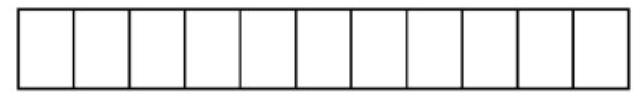
\includegraphics[max width=\textwidth, center]{2024_11_21_597e779fde37da7a0aa4g-22}

PESEL\\
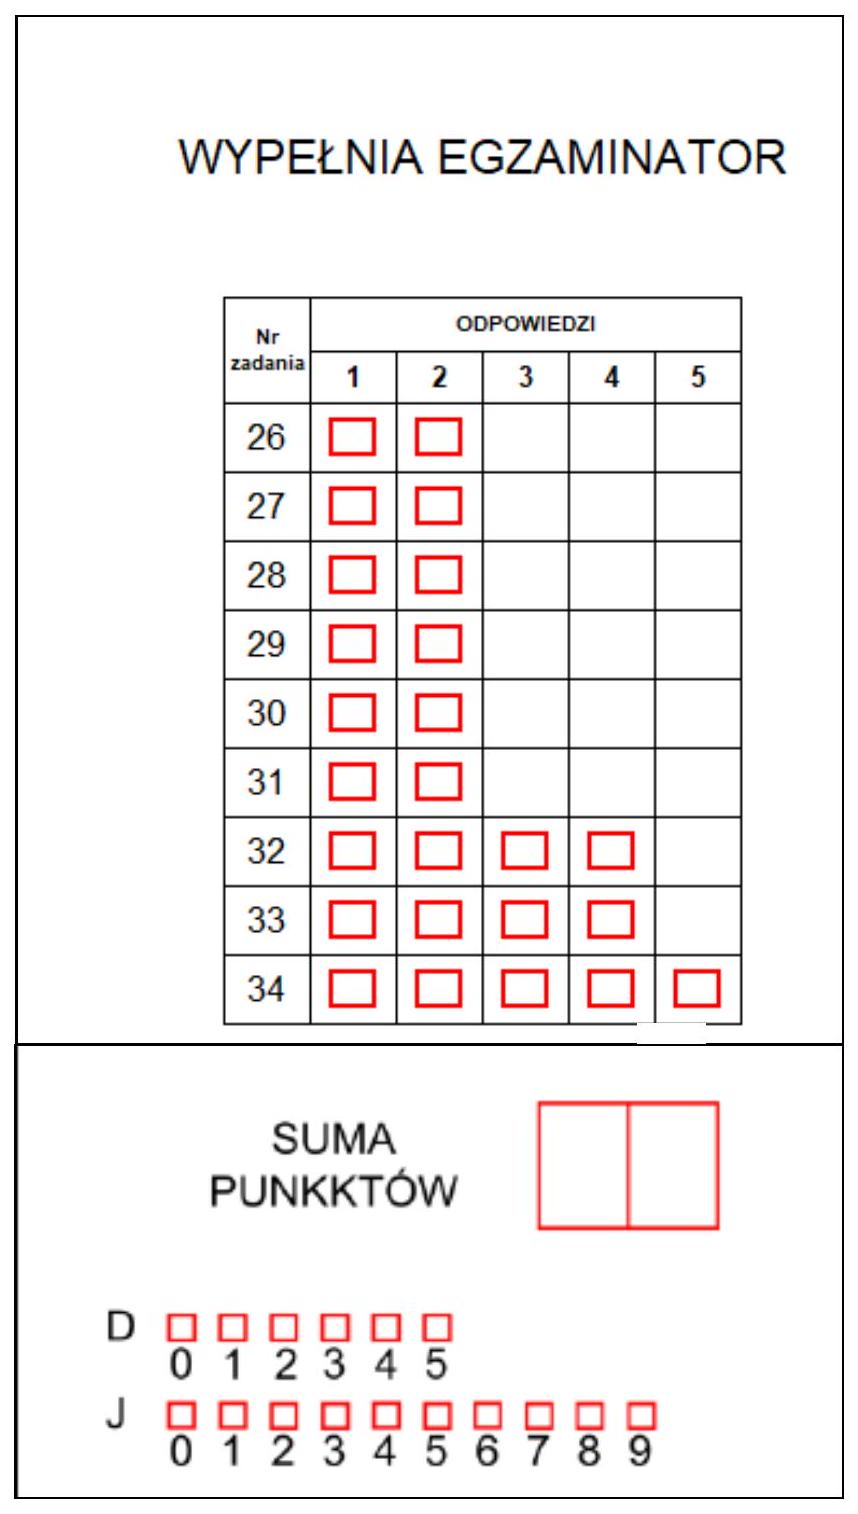
\includegraphics[max width=\textwidth, center]{2024_11_21_597e779fde37da7a0aa4g-22(1)}


\end{document}